%!TEX root = ../dissertation.tex
\chapter{Introduction}
\label{introduction}

We are currently experiencing a mass extinction event that parallels
other episodes in earth's history with high rates of biodiversity
decline \citep{Pimm1995, Dirzo2003, Schipper2008, Barnosky2011,
Dirzo2014}. Other than the five extinction events preceding it
\citep{Kolbert2014}, it is anthropogenic in origin \citep{Leakey1996,
Ceballos2015} and is associated with global warming \citep{Cook2016,
Wuebbles2017}, large-scale deforestation \citep{Wright2005}, destruction
of marine and freshwater habitats \citep{Burkhead2012}, and introduction
of invasive species \citep{Mooney2001}, all hallmarks of human
influence. Put shortly, the rate at which species go extinct is alarming
\citep{Newbold2016, Ceballos2017, Hallmann2017}, and our children will
likely experience a world with less than half the biodiversity we know
today. While this issue has raised the attention of country leaders and
conservation policies are being put in place worldwide
\citep{Puntaru2017}, this might not be enough to reverse the trend
without sustaining irreparable damage to the ecosystems of the planet.
To make matters worse, there are signs that the issue, despite its
urgency, is fading from public awareness \citep{Kusmanoff2017}. 

Conservation efforts require intimate knowledge of the systems they aim
to preserve: Of course, we cannot save what we do not know. The road
towards understanding the biology and the interaction of species is,
however, traveled on multiple levels. It is not enough to observe the
behaviour or the feeding preferences of an animal to understand the
impact of it being removed from its habitat. It is also not enough to
describe functional morphology to gain insight on ecological
implications. Neither is it sufficient to analyse the genes and draw
conclusions based on their composition and structure. Profound
understanding of any system can only be gained by studying it from
multiple angles and with interdisciplinary approaches. One such approach
is to sequence and analyse the genome of a species: the source code of
life that defines, by a manifold of means, its appearance, features,
behaviour and interactions with the environment.

The genome, that is, the entirety of DNA of an organism is a composition
of different functional complexes. It does not only contain genes, which
are translated into the proteins that make up cells and, ultimately, all
organisms; in fact, the human gene repertoire of around 23,000 genes
makes up only around 2 \% of the human genome \citep{Makalowski2001}
(Figure \ref{fig:human-genome}). The more prominent components of the
human genome include introns (non-coding sections of genes, \~26 \%),
but by far the most voluminous chunk consists of repetitive elements:
DNA segments that occur in sometimes many copies throughout the genome.
More than half of the human genome (52 \%) is occupied by repetitive
elements \citep{Lander2001}.  The major part of these repetitive
elements in the human genome, also called repeats, is formed by
transposable elements (45 \% of the genome).

\begin{figure}
\centering
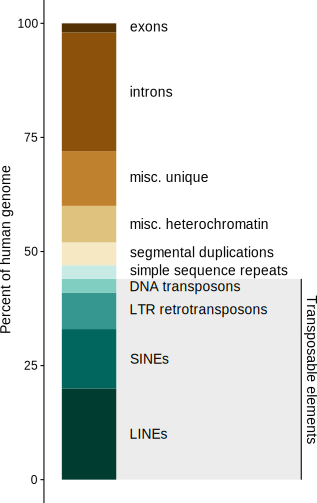
\includegraphics[width=0.3\textwidth]{human}
\caption{Composition of the human genome}
\label{fig:human-genome}
\end{figure}

Transposable elements are also known as ``jumping genes'' or ``parasitic
DNA''. 
